\documentclass[11pt]{article}
\usepackage{graphicx,amsmath,amsfonts,amssymb,graphicx} 
\usepackage[varg]{txfonts}
\usepackage{enumerate}
\usepackage{hyperref}
\usepackage{listings}
\usepackage{color}
\urlstyle{tt}
\usepackage{hyperref}
\usepackage{amsmath}
\usepackage{graphicx}
\usepackage{caption}
\usepackage{subcaption}
\usepackage[section]{placeins}
\renewcommand{\thesubsection}{\thesection.\alph{subsection}}
\usepackage{listings}
\usepackage{amssymb}
\usepackage{geometry}
\geometry{%
  letterpaper,
  lmargin=2cm,
  rmargin=2cm,
  tmargin=2cm,
  bmargin=2cm,
  footskip=12pt,
  headheight=12pt}
  


\usepackage{lastpage}
\usepackage{fancyhdr}

\title{\bf{CSE397: Assignment \#3}}
\author{Nicholas Malaya \\ Department of Mechanical Engineering \\
Institute for Computational Engineering and Sciences \\ University of
Texas at Austin} \date{} 


\def\squarebox#1{\hbox to #1{\hfill\vbox to #1{\vfill}}}
\def\qed{\hspace*{\fill}
        \vbox{\hrule\hbox{\vrule\squarebox{.667em}\vrule}\hrule}}
\newenvironment{solution}{\begin{trivlist}\item[]{\bf Solution:}}
                      {\qed \end{trivlist}}

\begin{document}
\maketitle
\newpage

\section*{ Problem 1}

\begin{enumerate}
\item [(A)] %PART A
For both $\mathcal{F}_{TN}$ and $\mathcal{F}_{TV}$ , derive the
      first-order necessary condition for optimality using calculus of
      variations, in both weak form and strong form. Use $\hat{u}$ to
      represent the variation of $u$. 

\begin{solution}
	To obtain the weak form for the Tikhonov regularization, take the variational derivative:
	\begin{align}
	\mathcal{F}_{TN}(u + \tau\hat{u}) &= \int_{\Omega}\left(u + \tau\hat{u} - u_0\right)^2d\mathbf{x}
		+ 0.5\int_{\Omega}
	 k(\mathbf{x})\nabla(u+\tau\hat{u})\cdot\nabla(u +
	 \tau\hat{u})d\mathbf{x}\nonumber \\ 
	\frac{d\mathcal{F}_{TN}}{d\tau} &= 2\int_{\Omega}\left(u + \tau\hat{u}-u_0\right)\hat{u}d\mathbf{x}
	    + \int_{\Omega} k(\mathbf{x})\nabla(u +
	 \tau\hat{u})\cdot\nabla\hat{u}d\mathbf{x}\nonumber\\ 
	\left.\frac{d\mathcal{F}_{TN}}{d\tau}\right|_{\tau=0} &=
	 2\int_{\Omega}\left(u -u_0\right)\hat{u}d\mathbf{x} +
	 \int_{\Omega} k(\mathbf{x})\nabla u
	 \cdot\nabla\hat{u}d\mathbf{x}\nonumber\\ 
    &= 0 \nonumber
	\end{align}
	Therefore the weak form for the Tikhonov regularization is given by:
	\begin{displaymath}
		2\int_{\Omega}\left(u -u_0\right)\hat{u}d\mathbf{x} + \int_{\Omega} k(\mathbf{x})\nabla u \cdot\nabla\hat{u}d\mathbf{x} = 0
	\end{displaymath}
	Then to obtain the strong form use Gauss Theorem:
	\begin{displaymath}
		2\int_{\Omega}\left(u -u_0\right)\hat{u}d\mathbf{x} - \int_{\Omega} \nabla \cdot (k(\mathbf{x})\nabla u)\hat{u}d\mathbf{x} + \int_{\Gamma} (k(\mathbf{x})\nabla u)\cdot n \hat{u}ds = 0 \hspace{1 cm} \forall\hat{u} \in H^1(\Omega)
	\end{displaymath}
	However it was prescribed that the Neumann condition on $u$ is zero, leaving:
	\begin{displaymath}
		2\int_{\Omega}\left(\left(u -u_0\right) - \nabla \cdot
	 (k(\mathbf{x})\nabla u)\right)\hat{u}d\mathbf{x}  = 0 \hspace{1
	 cm} \forall\hat{u} \in H^1(\Omega) 
	\end{displaymath}
	Since this is true for all variations $\hat{u}$ then the following strong form holds:
	\begin{align}
		2\left(u -u_0\right) - \nabla \cdot (k(\mathbf{x})\nabla u) &= 0 \nonumber \\
		\nabla u \cdot n &= 0 \nonumber
	\end{align} \\
	
	Following the same method for the modified total variational regularization:
	\begin{align}
	\mathcal{F}_{TV}^\epsilon(u + \tau\hat{u}) &= \int_{\Omega}\left(u + \tau\hat{u} - u_0\right)^2d\mathbf{x}
		+ \int_{\Omega}
	 k(\mathbf{x})\left(\nabla(u+\tau\hat{u})\cdot\nabla(u +
	 \tau\hat{u}) + \epsilon\right)^{0.5}d\mathbf{x}\nonumber \\ 
	\frac{d\mathcal{F}_{TV}^\epsilon}{d\tau} &= 2\int_{\Omega}\left(u + \tau\hat{u}-u_0\right)\hat{u}d\mathbf{x}
	    + \int_{\Omega} k(\mathbf{x})\frac{\left(\nabla(u+\tau\hat{u})\cdot\nabla\hat{u} \right)}{\sqrt{\left(\nabla(u+\tau\hat{u})\cdot\nabla(u + \tau\hat{u}) + \epsilon\right)}}d\mathbf{x}\nonumber\\
	\left.\frac{d\mathcal{F}_{TV}^\epsilon}{d\tau}\right|_{\tau=0}
	 &= 2\int_{\Omega}\left(u -u_0\right)\hat{u}d\mathbf{x} +
	 \int_{\Omega} k(\mathbf{x})\frac{\left(\nabla u
	 \cdot\nabla\hat{u} \right)}{\sqrt{\left(\nabla u\cdot\nabla u +
	 \epsilon\right)}}d\mathbf{x}\nonumber\\ 
    &= 0 \nonumber
	\end{align}
	This gives the weak form:
	\begin{displaymath}
	2\int_{\Omega}\left(u -u_0\right)\hat{u}d\mathbf{x} + \int_{\Omega} k(\mathbf{x})\frac{\left(\nabla u \cdot\nabla\hat{u} \right)}{\sqrt{\left(\nabla u\cdot\nabla u + \epsilon\right)}}d\mathbf{x} = 0 \hspace{1 cm} \forall\hat{u} \in H^1(\Omega) 
	\end{displaymath}
	The performing Gauss Theorem for the strong form:
	\begin{displaymath}
	2\int_{\Omega}\left(u -u_0\right)\hat{u}d\mathbf{x} 
	-\int_{\Omega} \nabla \cdot \left(k(\mathbf{x})\frac{\nabla
	 u}{\sqrt{\left(\nabla u\cdot\nabla u +
	 \epsilon\right)}}\right)\hat{u}d\mathbf{x} 
	+\int_{\Gamma} k(\mathbf{x})\hat{u}\frac{\nabla u \cdot n}{\sqrt{\left(\nabla u\cdot\nabla u + \epsilon\right)}}ds
	= 0 \hspace{1 cm} \forall\hat{u} \in H^1(\Omega) 
	\end{displaymath}
	Again the prescribed boundary condition on $\Gamma$ causes the boundary to be zero, leaving:
	\begin{displaymath}
	2\int_{\Omega}\left(u -u_0\right)\hat{u}
	- \nabla \cdot \left(k(\mathbf{x})\frac{\nabla
	 u}{\sqrt{\left(\nabla u\cdot\nabla u +
	 \epsilon\right)}}\right)\hat{u}d\mathbf{x} 
	= 0 \hspace{1 cm} \forall\hat{u} \in H^1(\Omega) 
	\end{displaymath}
	Since this holds for all variations $\hat{u}$ then the following strong form holds:
	\begin{align}
		2\left(u -u_0\right) - \nabla \cdot
	 \left(k(\mathbf{x})\frac{\nabla u}{\sqrt{\left(\nabla
	 u\cdot\nabla u + \epsilon\right)}}\right) &= 0 \nonumber\\ 
		\nabla u \cdot n &= 0 \nonumber
	\end{align}
\end{solution}

\item [(B)]%PART B
Show that when $\nabla u$ is zero, $\mathcal{R}_{TV}$ is not differentiable, but $\mathcal{R}^{\epsilon}_{TV}$ is.
\begin{solution}
	Performing the variational derivative of $\mathcal{R}_{TV}$ as done previously:
	\begin{align}
		\mathcal{R}_{TV}(u+\tau\hat{u}) &= \int_\Omega
	 k(\mathbf{x})\left(\nabla(u+\tau\hat{u}) \cdot
	 \nabla(u+\tau\hat{u})\right)^{0.5}d\mathbf{x} \nonumber \\ 
		\left.\frac{d\mathcal{R}_{TV}}{d\tau}(u+\tau\hat{u})\right|_{\tau = 0} &= \int_\Omega k(\mathbf{x})\frac{\nabla u \cdot \nabla\hat{u}}{\sqrt{\nabla u \cdot \nabla u}}d\mathbf{x} \nonumber
	\end{align}
	From here it is easy to see that a divide by 0 occurs if $\nabla
 u = 0$. Therefore the derivative of $\mathcal{R}_{TV}$ does not exist
 for $\nabla u = 0$. However for $\mathcal{R}^{\epsilon}_{TV}$, one has: 
	\begin{align}
		\mathcal{R}_{TV}^\epsilon(u+\tau\hat{u}) &= \int_\Omega k(\mathbf{x})\left(\nabla(u+\tau\hat{u}) \cdot \nabla(u+\tau\hat{u}) + \epsilon\right)^{0.5}d\mathbf{x} \nonumber \\
		\left.\frac{d\mathcal{R}^\epsilon_{TV}}{d\tau}(u+\tau\hat{u})\right|_{\tau
	 = 0} &= \int_\Omega k(\mathbf{x})\frac{\nabla u \cdot
	 \nabla\hat{u}}{\sqrt{\nabla u \cdot \nabla u +
	 \epsilon}}d\mathbf{x} \nonumber 
	\end{align}
	Then the derivative exists for $\nabla u = 0$ as the divide by 0
 is avoided due to the nonzero epsilon. 
\end{solution}

\item [(C)] %C
For both $\mathcal{F}_{TN}$ and $\mathcal{F}_{TV}^\epsilon$ , derive the
      infinite-dimensional Newton step, in both weak and strong
      form. For consistency of notation, please use $\tilde{u}$ as the
      differential of $u$ (i.e. the Newton step). The strong form of the
      second variation of $\mathcal{F}_{TV}^\epsilon$ will give an
      anisotropic diffusion operator of the form $-
      \nabla\cdot(A(u)\nabla \tilde{u})$, where $A(u)$ is an anisotropic
      tensor that plays the role of the diffusivity coefficient. (In
      contrast, you can think of the second variation of
      $\mathcal{F}_{TV}^\epsilon$ giving an isotropic diffusion
      operator, i.e. with $A = \alpha I$ for some $\alpha$.) 

\begin{solution}
	As shown in class the Newton step is given by:
	\begin{displaymath}
		\left.\frac{d\delta u\pi(u+\tau\tilde{u},\hat{u})}{d\tau}\right|_{\tau = 0} =
		-\left.\frac{d\pi(u+\tau\hat{u})}{d\tau}\right|_{\tau = 0}
	\end{displaymath}
	where the $\pi$ function will be either $\mathcal{F}_{TN}$ or
 $\mathcal{F}_{TV}^\epsilon$. However the left hand side needs to be
 evaluated for these cases. First for $\mathcal{F}_{TN}$: 
	\begin{align}
		\delta u\mathcal{F}_{TN}(u+\tau\tilde{u},\hat{u}) &=
		2\int_{\Omega}\left(u + \tau \tilde{u}
	 -u_0\right)\hat{u}d\mathbf{x} + \int_{\Omega}
	 k(\mathbf{x})\nabla(u+\tau\tilde{u})
	 \cdot\nabla\hat{u}d\mathbf{x} \\ 
		\frac{d
	 (\delta
	 u\mathcal{F}_{TN})}{d\tau}(u+\tau\tilde{u},\hat{u})|_{\tau =0} &=  
		2\int_{\Omega}\tilde{u}\hat{u}d\mathbf{x} +
	 \int_{\Omega} k(\mathbf{x})\nabla \tilde{u}
	 \cdot\nabla\hat{u}d\mathbf{x}
	\end{align}
The weak form is therefore, 
\begin{equation}
 2\int_{\Omega}\tilde{u}\hat{u}d\mathbf{x} +
  \int_{\Omega} k(\mathbf{x})\nabla \tilde{u}
  \cdot\nabla\hat{u}d\mathbf{x} = 2 \int_{\Omega}(u-u_0)\hat u dx +
  \int_{\Omega} k(x) \nabla u \cdot \hat u dx. 
\end{equation}

Then, $\mathcal{F}^{\epsilon}_{TV}$:
	\begin{align}
	 \delta u\mathcal{F}^{\epsilon}_{TV}(u+\tau\tilde{u},\hat{u}) &= 2\int_{\Omega}\left(u + \tau \tilde{u}
	 -u_0\right)\hat{u}d\mathbf{x} + \int_{\Omega} k(\mathbf{x})
	 \frac{\nabla(u+\tau\tilde{u})\cdot\nabla\hat{u}}{\sqrt{\nabla(u+\tau\tilde{u})\cdot\nabla(u+\tau\tilde{u})
	 +\epsilon}} dx \\ 
	 \frac{\delta
	 u\mathcal{F}^{\epsilon}_{TV}}{d\tau}(u+\tau\tilde{u},\hat{u})
	 &= 2\int_{\Omega}\tilde{u}\hat{u}d\mathbf{x}
	 + \int_{\Omega} k(\mathbf{x})
	 \frac{\nabla u \cdot\nabla\hat{u}}{\sqrt{\nabla(u+\tau\tilde{u})\cdot\nabla(u+\tau\tilde{u})
	 + \epsilon}} dx
	 - \int_{\Omega} k(\mathbf{x})\frac{
	 (\nabla (u+\tau \tilde u)\cdot \nabla \hat u) (\nabla (u+\tau
	 \tilde u)\cdot \nabla \tilde u)}
	 {(\sqrt{\nabla(u+\tau\tilde{u})\cdot\nabla(u+\tau\tilde{u}) 
	 + \epsilon)^{3/2}}} dx \\	 
	 \frac{\delta
	 u\mathcal{F}^{\epsilon}_{TV}}{d\tau}(u+\tau\tilde{u},\hat{u})
	 |_{\tau = 0} 
	 &= 2\int_{\Omega}\tilde{u}\hat{u}d\mathbf{x} +
	 \int_{\Omega} k(\mathbf{x})
	 \frac{\nabla \tilde u \cdot\nabla\hat{u}}{\sqrt{\nabla u \cdot
	 \nabla u +\epsilon}} dx
	 %
	 - \int_{\Omega} k(\mathbf{x})\frac{
	 (\nabla u \cdot \nabla u^T) (\nabla \tilde u \cdot \nabla \hat u)}
	 {(\sqrt{\nabla u \cdot\nabla u 
	 + \epsilon)^{3/2}}} dx 	
	\end{align}
The weak form is therefore, 
\begin{equation}
2\int_{\Omega}\tilde{u}\hat{u}d\mathbf{x} +
 \int_{\Omega} k(\mathbf{x})
 \frac{\nabla \tilde u \cdot\nabla\hat{u}}{\sqrt{\nabla u \cdot
 \nabla u +\epsilon}} dx
 %
 - \int_{\Omega} k(\mathbf{x})\frac{
 (\nabla u \cdot \nabla u^T) (\nabla \tilde u \cdot \nabla \hat u)}
 {(\sqrt{\nabla u \cdot\nabla u 
 + \epsilon)^{3/2}}} dx
 = 2 \int_{\Omega}(u-u_0)\hat u dx +  \int_{\Omega} k(\mathbf{x})
 \frac{\nabla u \cdot\nabla\hat{u}}{\sqrt{\nabla u \cdot
 \nabla u +\epsilon}} dx
\end{equation}

 We now have the weak forms for Newton steps of
 $\mathcal{F}_{TN}$ and $\mathcal{F}^{\epsilon}_{TV}$. Using Gauss'
 Theorem, and the condition that $\nabla \hat u \cdot n = 0$, we can
 regain the strong forms, namely: 
 \begin{align}
  2 \tilde u - \nabla \cdot (k(x)\nabla \tilde u) = 2(u-u_0) - \nabla
  \cdot (k(x)\nabla u)\\
  \nabla \hat u \cdot n = 0
 \end{align}
  and, 
 \begin{align}
  2 \tilde u - \nabla \cdot \left( \frac{k(x)}{(\nabla u \cdot \nabla u+
  \epsilon)^{1/2}} \left( I - \frac{1}{\nabla u \cdot \nabla u +
  \epsilon} \nabla u \cdot \nabla u^T \right) \nabla \tilde u \right) =
  2(u=u_0) - \nabla \cdot \left( \frac{k(x)}{(\nabla u \cdot \nabla u+
  \epsilon)^{1/2}} \nabla u \right) \\
  \nabla \hat u \cdot n = 0
\end{align}
\end{solution}

\item [(D)]
      Derive Expressions for the two eigenvalues and corresponding
      eigenvectors of A. Based on these expressions, given an
      explaination of why $\mathcal{F}^{\epsilon}_{TV}$ is effective at
      preserving sharp edges in the image, while $\mathcal{F}_{TN}$ is
      not. Consider a single Newton step for this argument. 

\begin{solution}
This problem is in two dimensions. Thus, our matrix is: 
\begin{equation*}
A(u) = \frac{k(x)}{(\nabla u \cdot \nabla u +
  \epsilon)^{1/2}}
  \left(
   \begin{array}{ c c }
    -\frac{u_x^2}{\nabla u \cdot \nabla u + \epsilon} + 1 &
     -\frac{u_x u_y}{\nabla u \cdot \nabla u + \epsilon} \\ 
    -\frac{u_x u_y}{\nabla u \cdot \nabla u + \epsilon}
      & -\frac{u_y^2}{\nabla u \cdot \nabla u + \epsilon} + 1
   \end{array} \right)
\end{equation*}
\end{solution}
      Now we need to only solve the characteristic equation of this matrix
      $A(u)$, which are, 
      \begin{equation*}
       \lambda = \frac{k(x)}{(\nabla u \cdot \nabla u +
	\epsilon)^{1/2}}, \frac{k(x)}{(\nabla u \cdot \nabla u +
	\epsilon)^{1/2}} \left(1-\frac{\nabla u \cdot \nabla u}{\nabla u
			  \cdot \nabla u + \epsilon}\right)
      \end{equation*}
      and the eigenvectors are: 
      \begin{equation}
        v=    
	 \left(
	  \begin{array}{ c }
	  u_y\\
	  -u_x 
	  \end{array}\right),
	 \left(\begin{array}{ c }
	  u_x\\
	  u_y 
	 \end{array}\right)
      \end{equation}
      This provides a clear picture as to why the
      $\mathcal{F}^{\epsilon}_{TV}$ method is more effective at
      preserving sharp edges. Near sharp edges, $\nabla u$ is
      large. When this goes to infinity, the Newton step eigenvalues
      will go to zero, locally. Since the second eigenvalue
      goes to zero there is little motion along its corresponding
      eigenvector, $\nabla u$. Therefore the edge will
      be preserved. This is not the case with $\mathcal{F}_{TN}$, as the
      eigenvalues of the matrix are $k(x)$ and will not be impacted by
      the gradient. 

\item [(D)]
      Show that for large $\epsilon$, $\mathcal{F}^{\epsilon}_{TV}$
      behaves like $\mathcal{F}_{TN}$, and for $\epsilon=0$, the Hessian
      of $\mathcal{F}^{\epsilon}_{TV}$ is singular. This suggests that
      $\epsilon$ should be small, but not too small. 

\begin{solution}
 First note that the Hessian of $\mathcal{F}^{\epsilon}_{TV}$ is the
 matrix A. Therefore for large $\epsilon$, the $\frac{\nabla u \cdot
 \nabla u}{\nabla u \cdot \nabla u + \epsilon}$ term will drop out 
 of the second eigenvalue of the Hessian. However then both eigenvalues
 of the k(x) Hessian of $\mathcal{F}^{\epsilon}_{TV}$ are 
 then $\frac{k(x)}{\nabla u \cdot \nabla u + \epsilon}$. This
 effectively causes the Hessian to be $\alpha I$ for 
 some $\alpha$. However if one takes $\epsilon$ to zero then the second
 eigenvalue goes to zero. Since one of the eigenvalues is zero, the
 Hessian is singular. 
\end{solution}

\end{enumerate}
%%%%%
%
%
%
%
\section*{ Problem 2}
\begin{itemize}
\item [(A)]
\begin{solution}
To derive the weak form we multiply by a test function $v$ and integrate by parts to get
\begin{eqnarray*}
 \int_{\Omega}fvdx&=&-\int_{\Omega}\nabla \cdot(A(x)\nabla u)vdx\\
&=&\int_{\Omega}A(x)\nabla u\cdot \nabla
 vdx-\int_{\partial\Omega}A(x)\nabla u \cdot n vds_x. 
\end{eqnarray*}
To incorporate the Dirichlet boundary conditions we assume that we can
 extend $u_0$ to a function $Eu_0$ on the whole domain $\Omega$. Then we
 can rewrite any solution $u$ as 
\begin{displaymath}
 u=Eu_0+w
\end{displaymath}
for a function $w$ that vanishes on the boundary $\partial
 \Omega$. Since we already know $Eu_0$ we are then left to find
 $w$. However, since we are now looking for a function $w$ that vanishes
 on the boundary, it is then also natural to choose the test functions
 in the same space as the functions we are seeking for. Hence, we arrive
 at the problem of finding $w$ with $w|_{\partial\Omega}=0$ such that 
\begin{displaymath}
 \int_{\Omega}A(x)\nabla (Eu_0+w)\cdot \nabla vdx= \int_{\Omega}fvdx
\end{displaymath}
for all $v$ such that $v|_{\partial\Omega}=0$. Note that the boundary
 integral vanishes in this case since we just consider test functions
 $v$ that vanish on the boundary. However, this can be reformulated as
 the problem of finding $w$ with $w|_{\partial\Omega}=0$ such that 
\begin{displaymath}
 \int_{\Omega}A(x)\nabla w\cdot \nabla vdx=
 \int_{\Omega}fvdx-\int_{\Omega}A(x)\nabla Eu_0\cdot \nabla vdx 
\end{displaymath}
for all $v$ such that $v|_{\partial\Omega}=0$.

This is the weak form. Since $A$ is symmetric
 and positive definite, this problem is equivalent to the minimization
 problem 
\begin{displaymath}
 \min_{u: u|_{\partial\Omega}=u_0} \frac{1}{2}\int_{\Omega}A(x)\nabla
 u\cdot \nabla udx-\int_{\Omega}fudx. 
\end{displaymath}
This is a well-known result in Functional analysis. However, let us
 justify this result. First, let us define the functional 
\begin{displaymath}
 \mathcal{F}(u):=\frac{1}{2}\int_{\Omega}A(x)\nabla u\cdot \nabla
 udx-\int_{\Omega}fudx. 
\end{displaymath}
Then we can compute the derivative
\begin{displaymath}
 \frac{\partial \mathcal{F}(u+\varepsilon \hat{u})}{\partial
 \varepsilon}|_{\varepsilon=0} 
\end{displaymath}
for all $\hat{u}$ that vanish on the boundary. Note that since we chose
 $\hat{u}$ in a way that it vanishes on the boundary, a necessary
 condition for the minimum is 
\begin{displaymath}
 \frac{\partial \mathcal{F}(u+\varepsilon \hat{u})}{\partial
 \varepsilon}|_{\varepsilon=0}=0 
\end{displaymath} 
for all $\hat{u}$ that vanish on the boundary. We already computed that
 condition in problem 1 and got that a minimizer $u$ has to satisfy 
\begin{displaymath}
 \int_{\Omega}A(x)\nabla u\cdot \nabla \hat{u}dx=
 \int_{\Omega}f\hat{u}dx 
\end{displaymath}
for all $\hat{u}$ that vanish on the boundary. However, this is exactly
 the weak formulation that we derived above. Hence, we know that any
 minimizer of the functional has to satisfy the weak formulation. 

The fact that the weak formulation is also a sufficient condition for
 $u$ to be a minimizer of the functional $\mathcal{F}$ is a little bit
 more subtle. This can be proved in a straight forward way by proving
 that for a solution of the weak formulation holds
\begin{displaymath}
 \mathcal{F}(u)\leq \mathcal{F}(u+w)
\end{displaymath}
for all $w$ that vanish on the boundary. An important assumption that
has to be made for this proof to work out is that $A$ is symmetric and
positive definite. 
\end{solution}

\item [(B)] Solve the problem in COMSOL using quadratic finite
      elements. 
\begin{solution}

 \begin{figure}[!htb]
        \centering
        \begin{subfigure}[bh]{0.45\textwidth}
                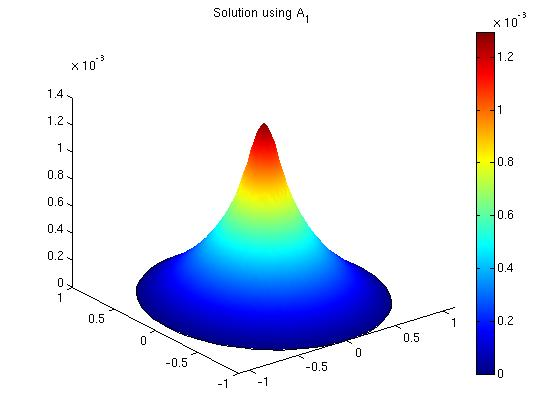
\includegraphics[width=\textwidth]{figs/prob2b1.jpg}
        \end{subfigure}%
        \begin{subfigure}[bh]{0.45\textwidth}
                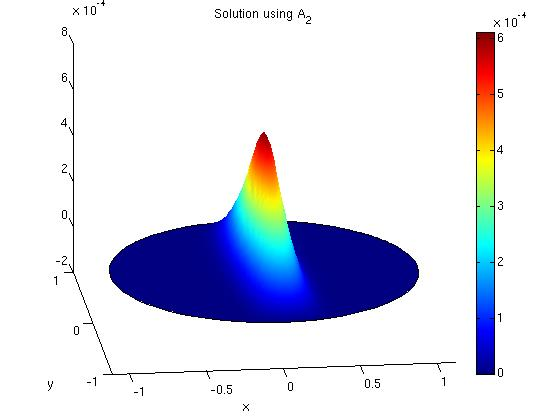
\includegraphics[width=\textwidth]{figs/prob2b2.jpg}
        \end{subfigure}
\end{figure}


In the first case the matrix is a scaled identity matrix meaning both
 directions have equal contributions. This is easily seen in the radial
 symmetry of the solution which is expected due to the forcing. However
 in the second matrix the y direction is dominant which is seen in
 disparity in size of the diagonal elements. This is reflected in the
 solution in which there is little change in the x direction while there
 are large shifts in the y direction. 
\end{solution}
\end{itemize}

\section*{ Problem 3}
\begin{itemize}
\item [(A)]
Compute a reconstruction using TN regularization. Since for TN
      regularization the weak form is linear (in u), you can use COMSOL
      linear solver femlin. Choose $\alpha >0$ such that you obtain a
      reasonable reconstruction , i.e., a reconstruction that removes
      noise from the image but also does not smooth the image too much.

\begin{solution}
 The optimal value alpha appears to be around $\alpha = 0.001$. Anything larger blurs more
 while anything less introduces noise similar to the noisy initial image.

 \begin{figure}[!htb]
        \centering
        \begin{subfigure}[bh]{0.45\textwidth}
                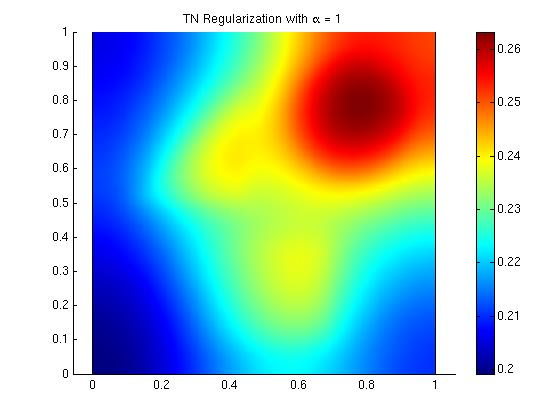
\includegraphics[width=\textwidth]{figs/prob3TNa1e0.jpg}
        \end{subfigure}%
        \begin{subfigure}[bh]{0.45\textwidth}
                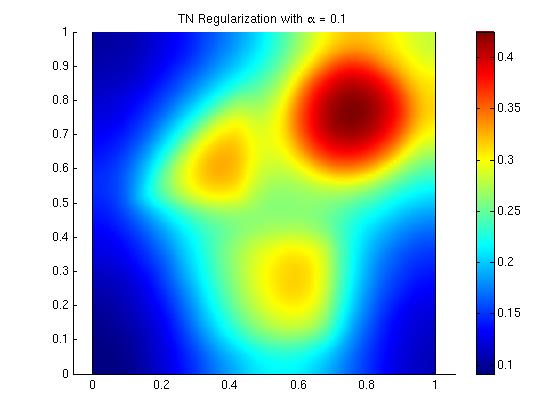
\includegraphics[width=\textwidth]{figs/prob3TNa1e-1.jpg}
        \end{subfigure}
        \centering
        \begin{subfigure}[bh]{0.45\textwidth}
                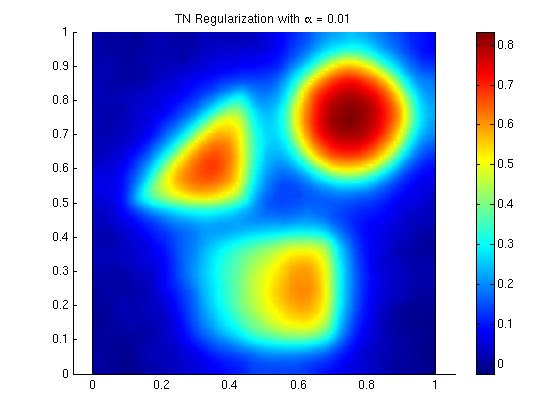
\includegraphics[width=\textwidth]{figs/prob3TNa1e-2.jpg}
        \end{subfigure}%
        \begin{subfigure}[bh]{0.45\textwidth}
                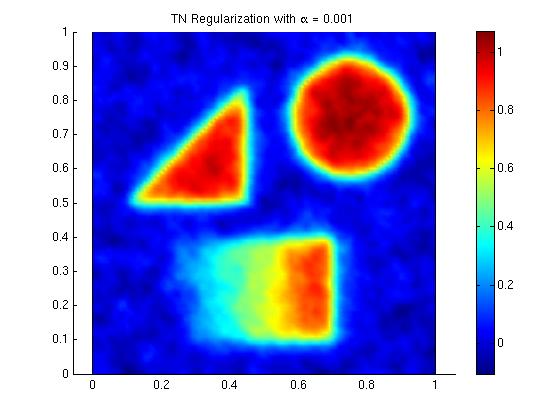
\includegraphics[width=\textwidth]{figs/prob3TNa1e-3.jpg}
        \end{subfigure}
        \centering
        \begin{subfigure}[bh]{0.45\textwidth}
                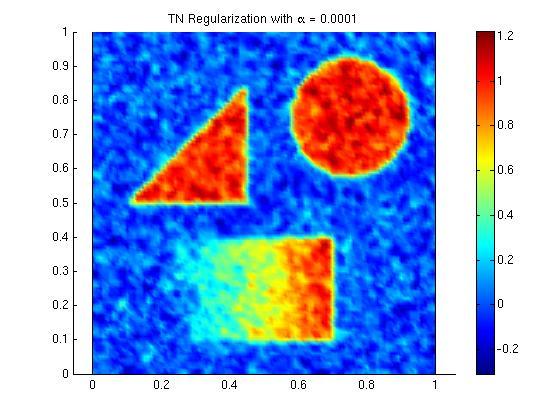
\includegraphics[width=\textwidth]{figs/prob3TNa1e-4.jpg}
        \end{subfigure}%
        \begin{subfigure}[bh]{0.45\textwidth}
                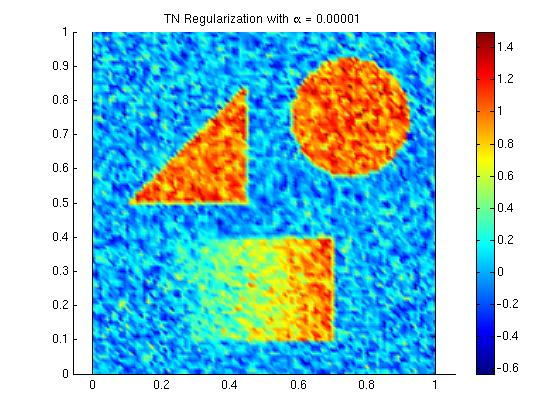
\includegraphics[width=\textwidth]{figs/prob3TNa1e-5.jpg}
        \end{subfigure}
\end{figure}

\end{solution}

\item [(B)]
\begin{solution}
 It is easy to see that the optimal alpha is near 0.01 since it
 has little effect on the blurring. Furthermore the number of iterations
 for chaging epsilon can be seen below. As epsilon goes to zero the
 number of steps increases as the matrix A becomes ill-conditioned as
 seen in Problem 1. However for large epsilon, the problem becomes more
 linear, requiring fewer steps to solve. 

 \begin{figure}[!htb]
        \centering
        \begin{subfigure}[bh]{0.45\textwidth}
                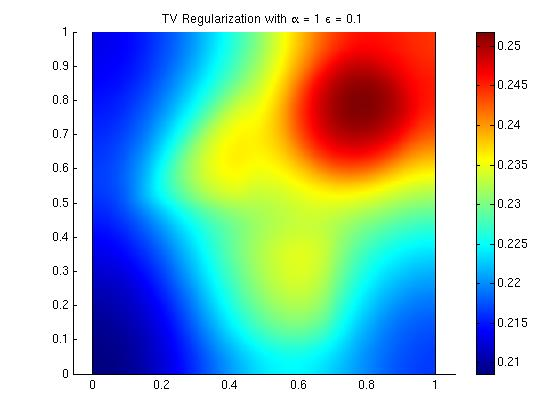
\includegraphics[width=\textwidth]{figs/prob3TVa1e0e1e-1.jpg}
        \end{subfigure}%
        \begin{subfigure}[bh]{0.45\textwidth}
                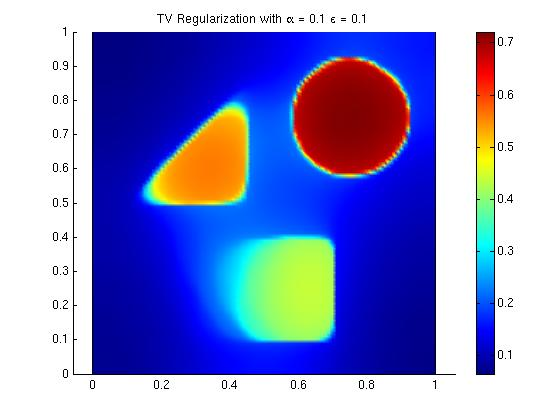
\includegraphics[width=\textwidth]{figs/prob3TVa1e-1e1e-1.jpg}
        \end{subfigure}
        \centering
        \begin{subfigure}[bh]{0.45\textwidth}
                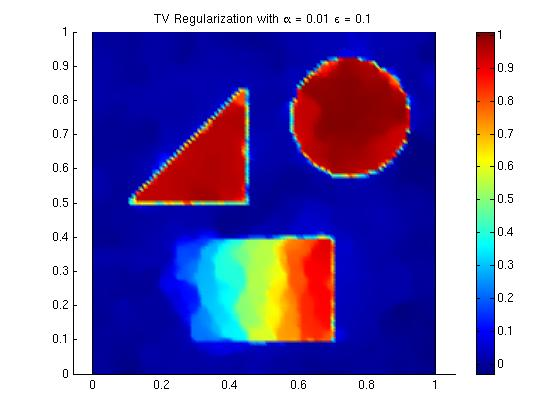
\includegraphics[width=\textwidth]{figs/prob3TVa1e-2e1e-1.jpg}
        \end{subfigure}%
        \begin{subfigure}[bh]{0.45\textwidth}
                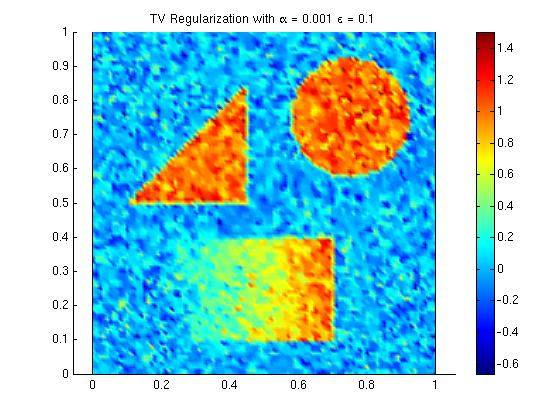
\includegraphics[width=\textwidth]{figs/prob3TVa1e-3e1e-1.jpg}
        \end{subfigure}
        \centering
        \begin{subfigure}[bh]{0.45\textwidth}
                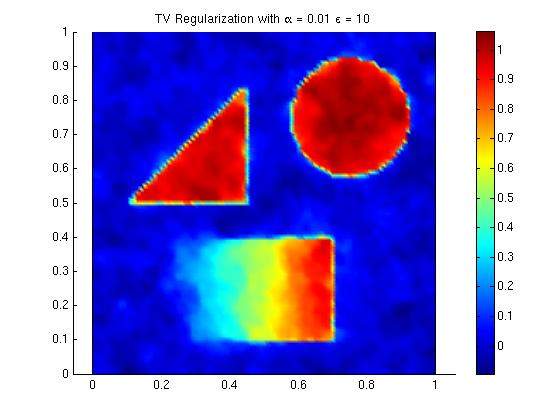
\includegraphics[width=\textwidth]{figs/prob3TVa1e-2e1e1.jpg}
        \end{subfigure}%
        \begin{subfigure}[bh]{0.45\textwidth}
                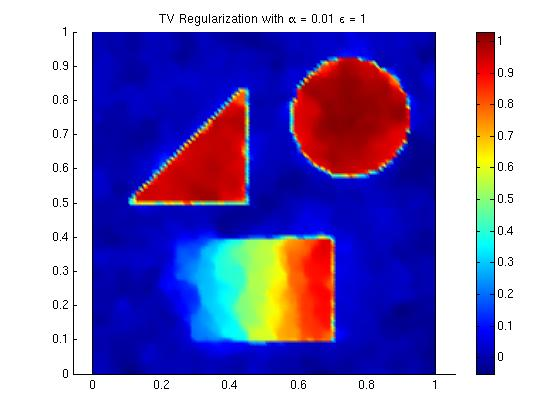
\includegraphics[width=\textwidth]{figs/prob3TVa1e-2e1e0.jpg}
        \end{subfigure}
\end{figure}

 \begin{figure}[!htb]
        \centering
        \begin{subfigure}[bh]{0.75\textwidth}
                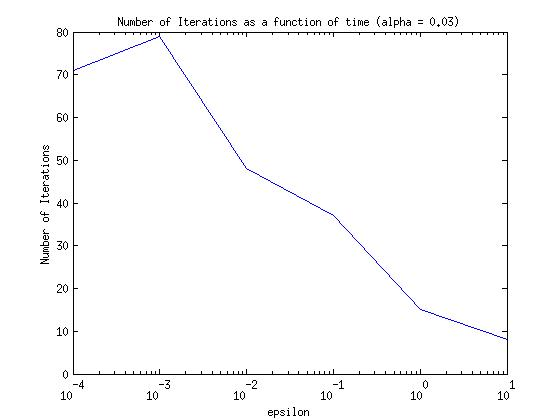
\includegraphics[width=\textwidth]{figs/iterationPlot.jpg}
        \end{subfigure}
\end{figure}


\end{solution}

\item [(C)]
\begin{solution}
 From the graphs above it is clear that the TV regularization preserves
 the sharp edges of the triangle and circle much better than then TN
 regularization. This is consistent with Problem 1. Also the TV
 regularization converged to the various extremes as predicted previously.
\end{solution}

\end{itemize}


\section*{Code}
Code for the first matrix in problem 2: 
\lstinputlisting{code/prob2b1.m}

\newpage
Code for the second matrix in problem 2:
\lstinputlisting{code/prob2b2.m}

\newpage 
This is the code for the Tikhonov regularization in Problem 3.
\lstinputlisting{code/TN.m}

\newpage 
This is the code for the Total Variation regularization in Problem 3.
\lstinputlisting{code/TV.m}

\newpage 
This is the code for determining the number of iterations for various epsilon in Problem 3.
\lstinputlisting{code/TVeps.m}

\end{document}


